\documentclass[naustrian]{beamer}
\usepackage[T1]{fontenc}
\usepackage[utf8]{inputenc}
\usepackage[ngerman]{babel}
\usetheme{metropolis}           % Use metropolis theme
\title{VIS: OPTICS$_\text{vis}$\\Milestone 4}
\date{\today}
\author{Group 11}
\institute{Fakultät für Informatik}
\titlegraphic{\hfill
\includegraphics[height=1cm]{img/uni_logo_farbe.pdf}}

\definecolor{asparagus}{rgb}{0.53, 0.66, 0.42}
\definecolor{alizarin}{rgb}{0.82, 0.1, 0.26}

\setbeamersize{description width=0.57cm}

\begin{document}
\maketitle

\begin{frame}{Agenda}
    \setbeamertemplate{section in toc}[sections numbered]
    \tableofcontents
\end{frame}

\section{Project definition}

\subsection{Motivation}

\begin{frame}{Project motivation}
    \begin{itemize}
        \item OPTICS: density based clustering
            \begin{itemize}
                \item algorithm jumps between points in some order
                \item records jump distances
            \end{itemize}
        \item output somewhat hard to read
            \begin{itemize}
                \item point order
                \item a list of numbers
            \end{itemize}
        \item staple visualization method: the bar chart
        \item[$\rightarrow$] more thorough and interactive visualization: OPTICSvis
    \end{itemize}
    \begin{figure}[h]
        \centering
        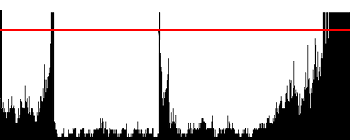
\includegraphics[height=.3\textheight]{img/optics-edited}
        \vspace{1em}
        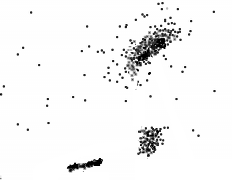
\includegraphics[width=.3\textwidth]{img/optics-edited-points-black}
    \end{figure}
\end{frame}

\subsection{Users and Tasks}

\begin{frame}{Users}
\begin{itemize}
 \item Teaching personnel
            \begin{itemize}
                \item for educational purposes
            \end{itemize}
  \item Researchers
            \begin{itemize}
                \item exploration
                \item testing before practical usage
            \end{itemize}
\item Anyone
            \begin{itemize}
                \item exploration
            \end{itemize}
  \end{itemize}
\end{frame}

\begin{frame}{Tasks}
\begin{itemize}
 \item Exploration
            \begin{itemize}
                \item get a feeling for the algorithm, get to know it
            \end{itemize}
 \item Education
  	\begin{itemize}
                \item learn about the algorithm and how to interpret the output
            \end{itemize}
  \item Testing
            \begin{itemize}
                \item give an idea if the algorithm fits the users problem
                \item see if result/output is satisfactory and useful
            \end{itemize}
  \end{itemize}
\end{frame}

{
\metroset{sectionpage=none}


\section{Approach}

\begin{frame}{Approach}
    \begin{itemize}
        \item static views (w/o interactive elements) provide an overview
        \item interaction can be used to filter or show more details on demand
        \item OPTICS is density-based: visualize densities
        \item make reachability chart interactive: draggable cutoff bar
        \item heat map makes cluster structures easier to see
        \item allow user to trace the algorithm
        \item attempt to visualize hierachy
    \end{itemize}
\end{frame}

\begin{frame}{Implementation}
    \begin{figure}[H]
        \centering
        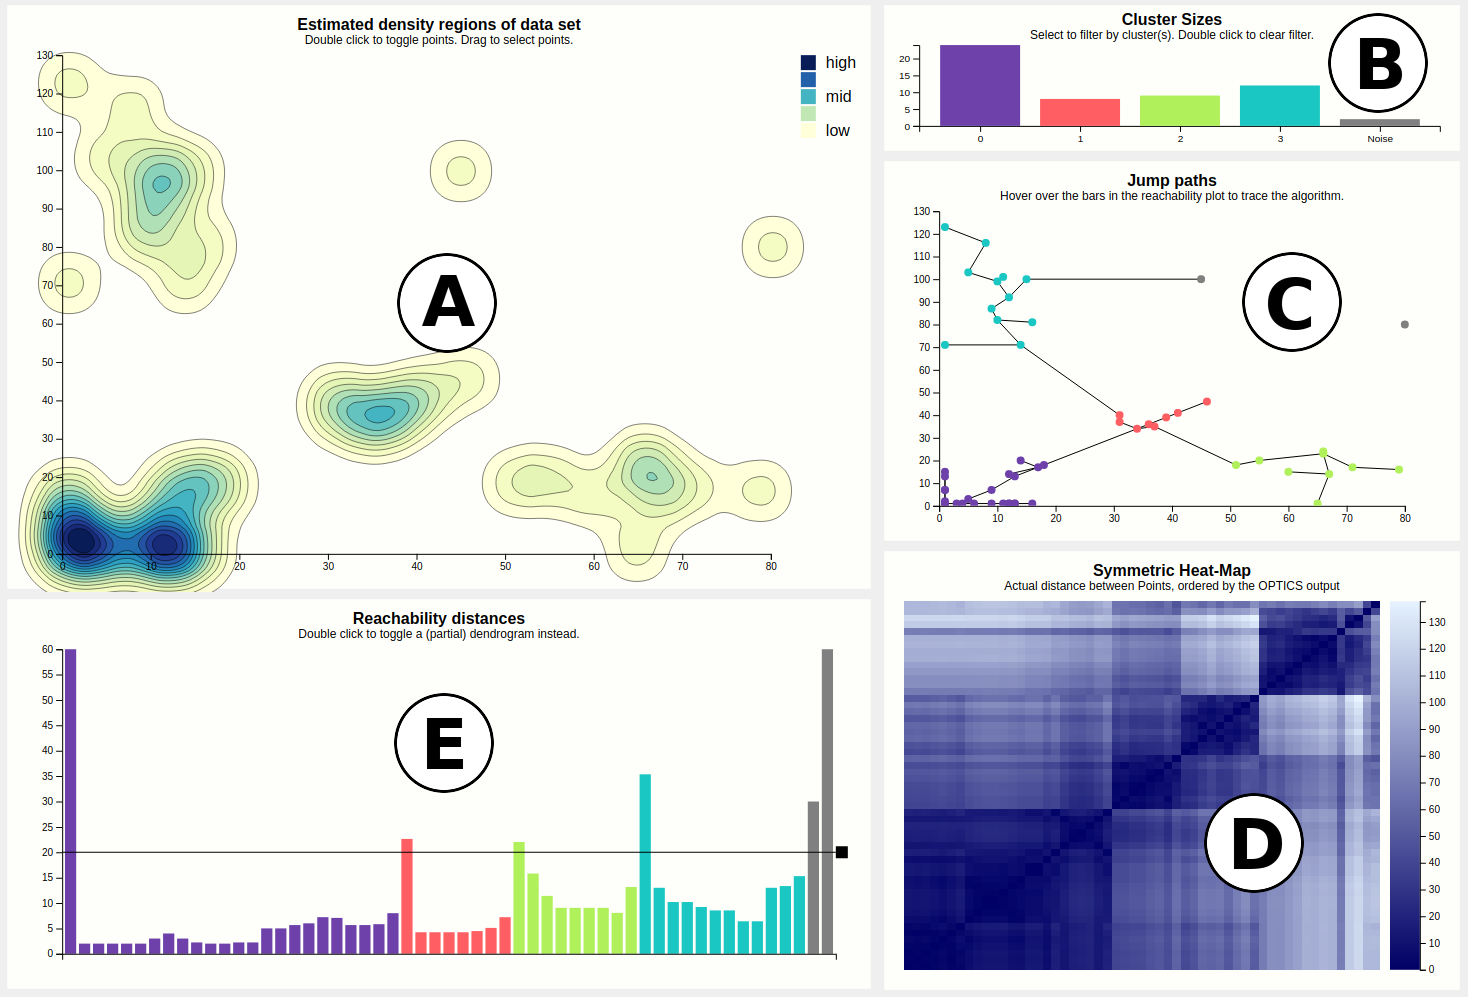
\includegraphics[height=0.85\textheight]{img/opticsvis-overview}
    \end{figure}
\end{frame}

\section{Demo}
}

\plain{Demo}

\section{Results}

\begin{frame}{Results}
    \begin{itemize}
        \item feedback overall favorable
        \item secondary cutoff bar was considered superfluous and confusing, removed in final prototype
        \item performance issues were prominent
        \item people tended to use the tool in a very superficial way, not very conclusive
        \item OPTICS basics needed to be taught beforehand
    \end{itemize}
\end{frame}

\section{Analysis}

\begin{frame}{Analysis}
    \begin{itemize}
        \item strengths
            \begin{itemize}
                \item[\color{asparagus}+] quick exploration of different aspects of OPTICS
                \item[\color{asparagus}+] good companion for teaching OPTICS
            \end{itemize}
        \item weaknesses
            \begin{itemize}
                \item[\color{alizarin}--] some previous knowledge of OPTICS needed
                \item[\color{alizarin}--] multidimensional data visualization could be improved
                \item[\color{alizarin}--] performance issues
            \end{itemize}
    \end{itemize}
\end{frame}

\plain{Thanks for your attention!}

\end{document}
